\part{Viola-Jones algoritam}\label{viola_jones_algorithm}

\section{Uvod} \label{viola_jones_introduction}

Namena algoritma je detekcija i lokalizacija objekata na slici. Osmišljen od
strane Paul Viola i Michael Jones 2001. godine \cite{Viola2001RapidOD}.

Dugo godina je zbog brze i pouzdane detekcije bio standardan način detekcije
lica na slici. I danas je prisutan u velikom broju mobilnih telefona i
digitalnih kamera, ali danas postaje polako zamenjen konvolucionim neuronskim
mrežama. \\

Pouzdanost i brzina su postignuti uvođenjem tri ključna doprinosa:
\begin{itemize}

\item \textbf{Integralna slika} omogućava brzo izračunavanje obeležja.
\item \textbf{AdaBoost} algoritam za učenje, odabiranjem obeležja povećava
  brzinu i pouzdanost detekcije.
\item \textbf{Kaskadni klasifikator} organizovanjem obeležja u kaskadama
  omogućava brzo odbacivanje pozadine slike. \\
\end{itemize}


\subsection{Integralna slika} \label{ii_sec}

Kao jedan od ključnih delova algoritma, integralna slika omogućava izračunavanje
površine svakog pravouganog obeležja u konstantnom vremenu.

Intenzitet piksela u integralnoj slici na poziciji x,y je zbir svih piksela koji
se nalaze gore i levo od pozicije x,y.

\begin{equation}
  \Scale[1.4]{ii(x,y)=\sum\limits_{x'\leq x, y'\leq y} i(x',y')}
  \label{IntegralImage_eq1}
\end{equation}

Gde je ii(x,y) integralna slika, a i(x,y) originalna slika. \\

\begin{figure}[h]
  \centering
  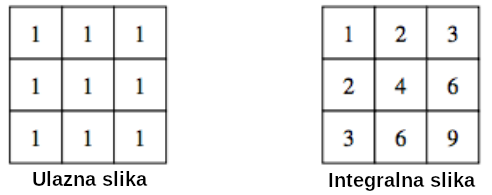
\includegraphics[width=8cm]{integral_image1}
  \caption{Primer integralne slike}
  \label{IntegralImage_img1}
\end{figure}

Piksele integralne slike je moguće računati u paraleli, ili
sekvencijalno. Izbor algoritma za računanje integralne slike značajno utiče na
performanse i potrebne hardverske resurse. \\
U paralelnoj implementaciji cena je
više pristupa memoriji i više potrebnih sabirača, dok je kod sekvencijalne
implementacije manja brzina proračunavanja. \\

Osobina koja integralnu sliku čini pogodnu za korišćenje u Viola-Jones algoritmu
je da je za računanje bilo koje pravougaone površine unutar integralne slike
potrebno 2 oduzimanja i 1 sabiranje.

\begin{figure}[h]
  \centering
  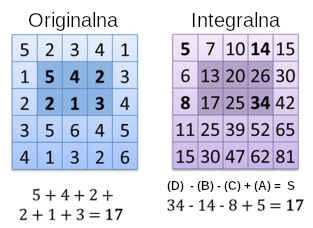
\includegraphics[width=8cm]{integral_image2}
  \caption{Primer računanja površine pravougaonika \cite{IntegralImage1_web}}
  \label{IntegralImage_img2}
\end{figure}

Na slici (\ref{IntegralImage_img2}) je prikazano računanje površine pravougaonika na
originalnoj slici i na integralnoj slici.
Kao što se može videti za površinu pravougaonika MxN na originalnoj slici nam je
potrebno MxN-1 sabiranja. \\
Dok je kod integralne slike broj operacija 2 oduzimanja i 1 sabiranje i ne zavisi od dimenzija pravougaonika.

\begin{equation}
  \Scale[1.4]{\sum\limits_{(x,y)\in ABCD} i(x,y)=ii(D)+ii(A)-ii(B)-ii(C)}
  \cite{Cen2016StudyOV}
  \label{IntegralImage_eq2}
\end{equation}

\newpage

\subsection{AdaBoost i HAAR obeležja}

\subsubsection{HAAR obeležja}

Detekcija na slici se vrši na prozorima manjih dimenzija. Na ovim prozorima
računaju se HAAR obeležja koja se sastoje od dva ili više pravougaonika, kao na
slici (\ref{haar_features_img1}). \\
Svako obeležje se računa sabiranjem piksela crnih pravougaonika potom
oduzimanjem zbira piksela belih pravougaonika. \\
Reprezentacija prozora pomoću integralne slike omogućava da se obeležja izračunavaju u konstantnom vremenu.

\begin{figure}[h]
  \centering
  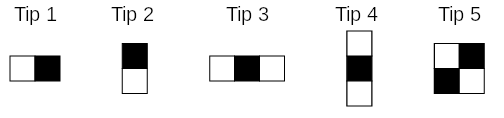
\includegraphics[width=12cm]{haar_features1}
  \caption{HAAR obeležja \cite{Jensen2008ImplementingTV}}
  \label{haar_features_img1}
\end{figure}

Dimenzije prozora se razlikuju od modela klasifikatora. Jedan
često korišćeni model koristi prozor dimezije 24x24. \\

\begin{figure}[h]
  \centering
  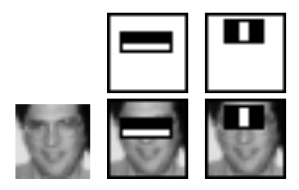
\includegraphics[width=8cm]{haar_features2}
  \caption{Primer obeležja za detekciju lica \cite{Viola2001RapidOD}}
  \label{haar_features_img2}
\end{figure}

Oblik odabranih obeležja će zavisiti od namene detektora, na
slici(\ref{haar_features_img2}) se mogu videti dva tipična obeležja koja su od
interesa za detekciju lica. \\
Prvo obeležje namenjeno je merenju razlike
intenziteta regiona čela i očiju. Obeležje koristi činjenicu da je oblast čela
svetlija od očiju. \\
Dok drugo obeležje poredi intenzitet regiona mosta nosa sa očima. \\

Kako su obeležja od interesa koja se koriste u modelima na
slici(\ref{haar_features_img1}).
Za datu dimenziju prozora kombinacije svih mogućih varijacija oblika i pozicija
datih obeležja čini skup od 160.000 različitih obeležja.
Kako je većina ovih obeležja slična i davaće slične rezultate, ovaj broj se može
drastično smanjiti korišćenjem algoritma za učenje AdaBoost.

\subsubsection{AdaBoost}

Kako je već rečeno može se dobiti oko 160.000 obeležja za prozor dimenzije
24x24. Od ovog broja samo neka obeležja mogu dati dobre rezultate prilikom
detekcije, kao na slici(\ref{haar_features_img2}) u primeru detektora lica. \\

Kako bi se odabrao skup korisnih obeležja može se koristiti neki od algoritama
mašinskog učenja. Viola i Jones predlažu modifikovani AdaBoost algoritam. \\

Ideja AdaBoost-a je kombinovanje više \emph{weak learner}-a kako bi se dobila
pouzdana detekcija. \\
\emph{Weak learner} je kalsifikator koji ima pouzdanost pogađanja malo bolju
nego nasumičnu. Odnosno pouzdanost \emph{weak learner}-a mora biti bar malo
iznad 50\%. \\

Kombinacijom ovako dobijenih \emph{weak learner}-a može se dobiti \emph{strong
  classifier} \\

Kao rezultat AdaBoost algoritma dobićemo skup obeležja, u ovom radu se koristi
model sa skupom od 2913 obeležja.

\newpage

\subsection{Kaskadni klasifikator}

Osnovni princip Viola-Jones algoritma je da se na osnovu svih obeležja u modelu dobije informacija da li se na
trenutnom položaju prozora nalazi traženi objekat (npr. lice).\\
Kako na slici većina skeniranih regiona ne sadrži lice, računanje svih obeležja
na svakoj poziciji bi bilo suvišno. Tako da je korišćenje jednog jakog
klasifikatora neefikasno. \\

Ideja obrazovanja kaskadnog klasifikatora je da se prozori na kojima se očigledno ne nalazi lice odbace
brzo, nakon samo nekoliko izračunatih obeležja.

\begin{figure}[h]
  \centering
  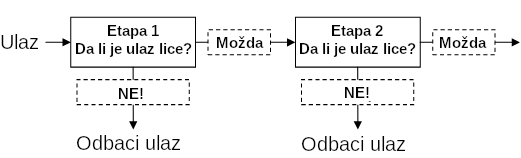
\includegraphics[width=14cm]{cascade_classifier1}
  \caption{Kaskadni klasifikator \cite{Jensen2008ImplementingTV}}
  \label{cascade_classifier_img1}
\end{figure}

Kako bi se prozori bez lica brzo odbacili predlog je da se jaki klasifikatori
grupišu u etape (eng. \emph{stage}). Svaka etapa treba da bude dobra u
odlučivanju da li se na analiziranom prozoru definitivno ne nalazi lice. Ukoliko
je to slučaj taj prozor će se brzo odbaciti. \\
Ukoliko rezultat etape ukazuje na to da se na prozoru možda nalazi lice, preći
će se na izvršavanje sledeće etape. \\

Konačno ukoliko sve etape u klasifikatoru na analiziranom prozoru daju rezultat da se možda nalazi
lice, može se zaključiti da se na toj poziciji zaista nalazi lice. \\
Zahvaljujući ovome postiže se veoma pouzdan klasifikator sa malim procentnom
pogrešno negativnih (eng. \emph{false negative}) rezultata na krajnjim etapama. \\

Kao primer u ovom radu će se koristiti model kaskadnog klasifikatora za
prepoznavanje lica, sa 25 etapa i 2913 obeležja raspoređenih po etapama. \\
U prvoj etapi se nalazi samo 9 obeležja, dok taj broj raste do 211 u kasnijim etapama.

\newpage

\begin{figure}[h]
  \centering
  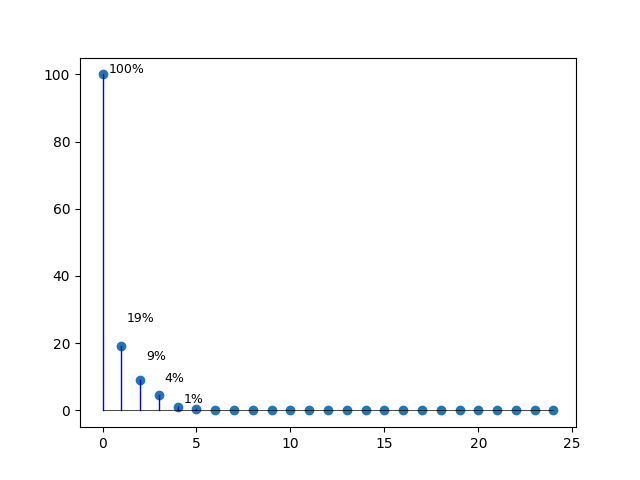
\includegraphics[width=12cm]{cascade_classifier2}
  \caption{Procenat prolaska etapa}
  \label{cascade_classifier_img2}
\end{figure}

Na slici(\ref{cascade_classifier_img2}) je prikazana statistika izvršavanja
etapa na \emph{Caltech Dataset-u}\cite{CALTECH_DATASET}, koji sadrži 450 slika
od 27 različitih ljudi pod različitim osvetljenjima, izrazima i pozadinama. \\

Vrednosti različitih tačaka na grafu predstavlja procenat izvršavanja date etape
na svih 450 slika. Prva etapa će se naravno uvek izvršiti, dok će se druga etapa
izvršiti samo u 19\% analiziranih prozora, druga 9\% itd... \\
Vidimo da je posle pete etape procenat izvršavanja manji od 1\%. \\

\newpage

\subsection{Invarijantnost veličine}\label{image_scaling}

Kako lica na slikama mogu biti bliže ili dalje kameri odnosno mogu biti
različitih dimenzija, potrebno je obezbediti da se ona detektuju nezavisno od
veličine. \\

Pošto su obeležja istrenirana da detektuju samo lica koja su iste dimenzije kao
i veličina obeležja potrebno je obezbediti skaliranje slike ili obeležja kako bi
mogli da detektujemo lica veća od dimenzije obeležja. \\
Pri čemu je najmanja dimenzija lica koje je moguće detektovati jednaka dimenziji obeležja.

\begin{figure}[h]
  \centering
  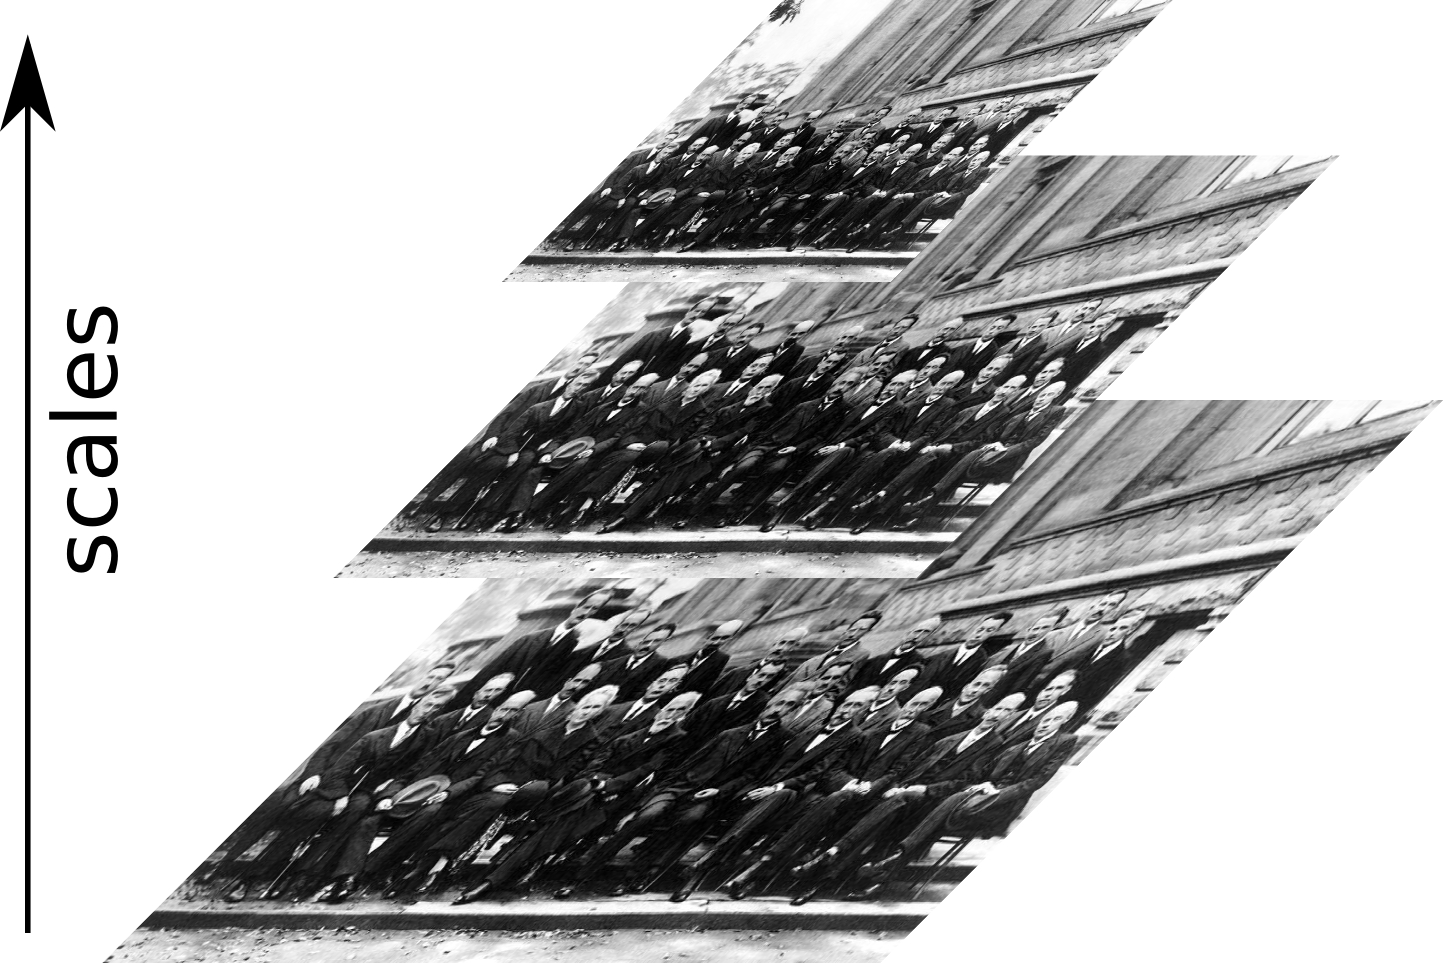
\includegraphics[height=5cm]{image_pyramid}
  \caption{Piramida slike\cite{ImagePyramid_web}}
  \label{image_pyramid}
\end{figure}

Ovo je rešeno uvođenjem skaliranja slike. Kao na slici(\ref{image_pyramid}) prvo
je potrebno odraditi detekciju na originalnoj slici, zatim se slika smanjuje sa
nekim faktorom i ponovo se vrši detekcija.
Skaliranje se vrši sve dok je dimenzija skalirane slike veća od dimenzije obeležja.

\begin{figure}[h]
  \centering
  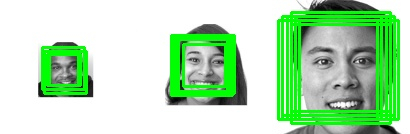
\includegraphics[width=12cm]{sixfaces_scaled_res}
  \caption{Različite veličine lica}
  \label{sixfaces_scaled}
\end{figure}

Na slici(\ref{sixfaces_scaled}) može se videti rezultat klasifikatora za 3 lica
različitih dimenzija. \\

\newpage

\subsection{Invarijantnost osvetljaja}\label{lumi_inv_sec}

Lica se mogu naći pod raznim osvetljenjima što uzrokuje problem ovom algoritmu.


\begin{figure}[!htb]
\centering
\parbox{6cm}{
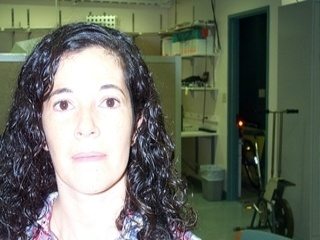
\includegraphics[width=6cm]{overexposed_light}
\caption{Previše osvetljaja\cite{CALTECH_DATASET}}
\label{overexposed_light}}
\qquad
\begin{minipage}{6cm}
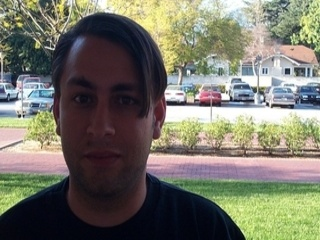
\includegraphics[width=6cm]{underexposed_light}
\caption{Premalo osvetljaja\cite{CALTECH_DATASET}}
\label{underexposed_light}
\end{minipage}
\end{figure}

Na slikama(\ref{overexposed_light}, \ref{underexposed_light}) su prikazane dve
slike koje zbog nepovoljnog osvetljenja nisu detektovane od strane
klasifikatora.
Slika(\ref{overexposed_light}) nije detektovana zbog prevelikog osvetljenja
lica, dok Slika(\ref{underexposed_light}) nije detektovana zbog slabog
osvetljenja.  \\

Kao delimično rešenje ovog problema uvedeno je računanje standardne devijacije
prozora koji se detektuje.
Ovo može poboljšati detekciju u nekim slučajevima, ali ne i ekstremnim kao u
prethodnom primeru.

\subsection{Varijantnost rotacije}

\begin{figure}[!htb]
\centering
\parbox{6cm}{
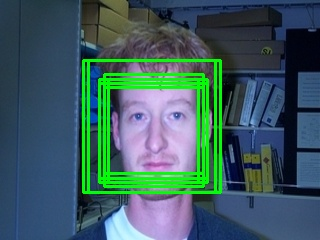
\includegraphics[width=6cm]{rotation_variance}
\caption{Ne rotirana\cite{CALTECH_DATASET}}
\label{rotation_variance}}
\qquad
\begin{minipage}{6cm}
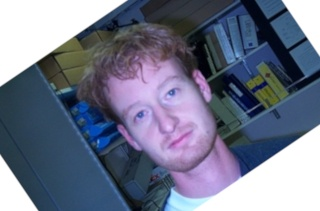
\includegraphics[width=6cm]{rotated_res}
\caption{Rotirana\cite{CALTECH_DATASET}}
\label{rotated_res}
\end{minipage}
\end{figure}